\chapter{Тестирование разработанного программного комплекса}

Разработанная система, реализующая описанные методы, первоначально испытывалась с использованием синтетических тестов, разработанных специально для тестирования корректности реализации. Однако синтетические тесты зачастую не отражают реальное качество анализатора в связи с ограниченностью возможных синтаксических конструкций, а также ввиду ограниченного объёма тестирующего кода. Кроме того, синтетические тесты не позволяют исследовать такие показатели разработанных методов, как масштабируемость и производительность анализатора. Наконец, поскольку разработанный комплекс предполагается к внедрению и промышленному использованию, имеет смысл произвести тестирование на наиболее характерных проектах. В связи с этим возникает необходимость проведения тестирования с использованием кода реальных проектов.

\section{Выбор тестовых проектов}

Для тестирования системы и оценки её количественных и качественных характеристик можно выбрать ряд пакетов различного размера. Желательно также, чтобы среди выбранных проектов присутствовал ряд проектов, не проходивших ранее проверку с использованием известных статических анализаторов. Поскольку после проверки другими статическими анализаторами и исправления найденных ошибок уменьшается количество потенциальных положительных срабатываний, результаты тестирования будут искажены. С другой стороны, вопрос взаимодействия с другими статическими анализаторами также интересен и представляет практический интерес, поскольку для поиска дефектов в разрабатываемом программном коде зачастую используется не один, а несколько анализаторов, причём как статических, так и динамических. Особенный интерес представляет возможность нахождения дефектов после проверки другими анализаторами, поскольку это свидетельствует о возможности дополнения существующих анализаторов или их замены. Это позволит провести сравнение результатов разработанного комплекса на проектах, прошедших статический анализ ранее, и проектах, его не проходивших.


Что касается крупных програмных комплексов, то на данную роль была отобрана ОС Android. Данная ОС включает в себя 389 пакетов, связанный между собой, и имеет суммарный объём анализируемого кода на языках C и C++ около 10 млн. SLoc. Кроме того, данный программный комплекс включает многие из уже описанных ранее пакетов, что позволяет заменить данным комплексом остальные, которые уже входят в его состав. Особый интерес для тестирования представляет то обстоятельство, что ОС Android может собираться для разных архитектур (x86, x86\_64, ARM и MIPS), причём  исполняемые файлы различных архитектур могут генерироваться во время одной сборки. Большое количество межфайловых связей делают проект интересным для межмодульного анализа и исследования масштабируемости разработанных методов межпроцедурного анализа. Общие характеристики исходного кода ОС Android приведены в таблицах \ref{table:android-char} и \ref{table:android-code}.

\begin{table} [htbp]
  \centering
  \parbox{15cm}{\caption{Характеристики тестовой базы ОС Android}\label{table:android-char}}
%  \begin{center}
  \begin{tabular}{| p{0.6\linewidth} || p{0.3\linewidth} |}
  \hline
  \hline
  Характеристика   & Значение \\
  \hline
  \hline
  Количество строк кода   & 10 млн \\
  \hline
  Количество файлов исходного кода      & 31038    \\
  \hline
  Количество транслируемых модулей  & 20635   \\
  \hline
  Количество архитектур на построение & 2   \\
  \hline
  Количество пакетов & 389 \\
  \hline
  \hline
  \end{tabular}
%  \end{center}
\end{table}

\begin{table} [htbp]
  \centering
  \parbox{15cm}{\caption{Код ОС Android на языках C и C++}\label{table:android-code}}
%  \begin{center}
  \begin{tabular}{| l | l | l | l | l |}
  \hline
  \hline
  Тип файла   & Файлов   & Пустых строк   & Комментариев & Строк кода \\
  \hline
  \hline
  Код C++                  & 18007  & 950783     &    952630   &   5036304 \\
  \hline
  Код C                    & 13031  & 783549     &   1056897   &   4711475 \\
  \hline
  Header                   & 26669  & 690283     &    1375129  &   2659402 \\
  \hline
  Всего                    & 57707  & 2424615    &    3384656  &   12407181 \\
  \hline
  \hline
  \end{tabular}
%  \end{center}
\end{table}

\begin{figure}
   \centering
   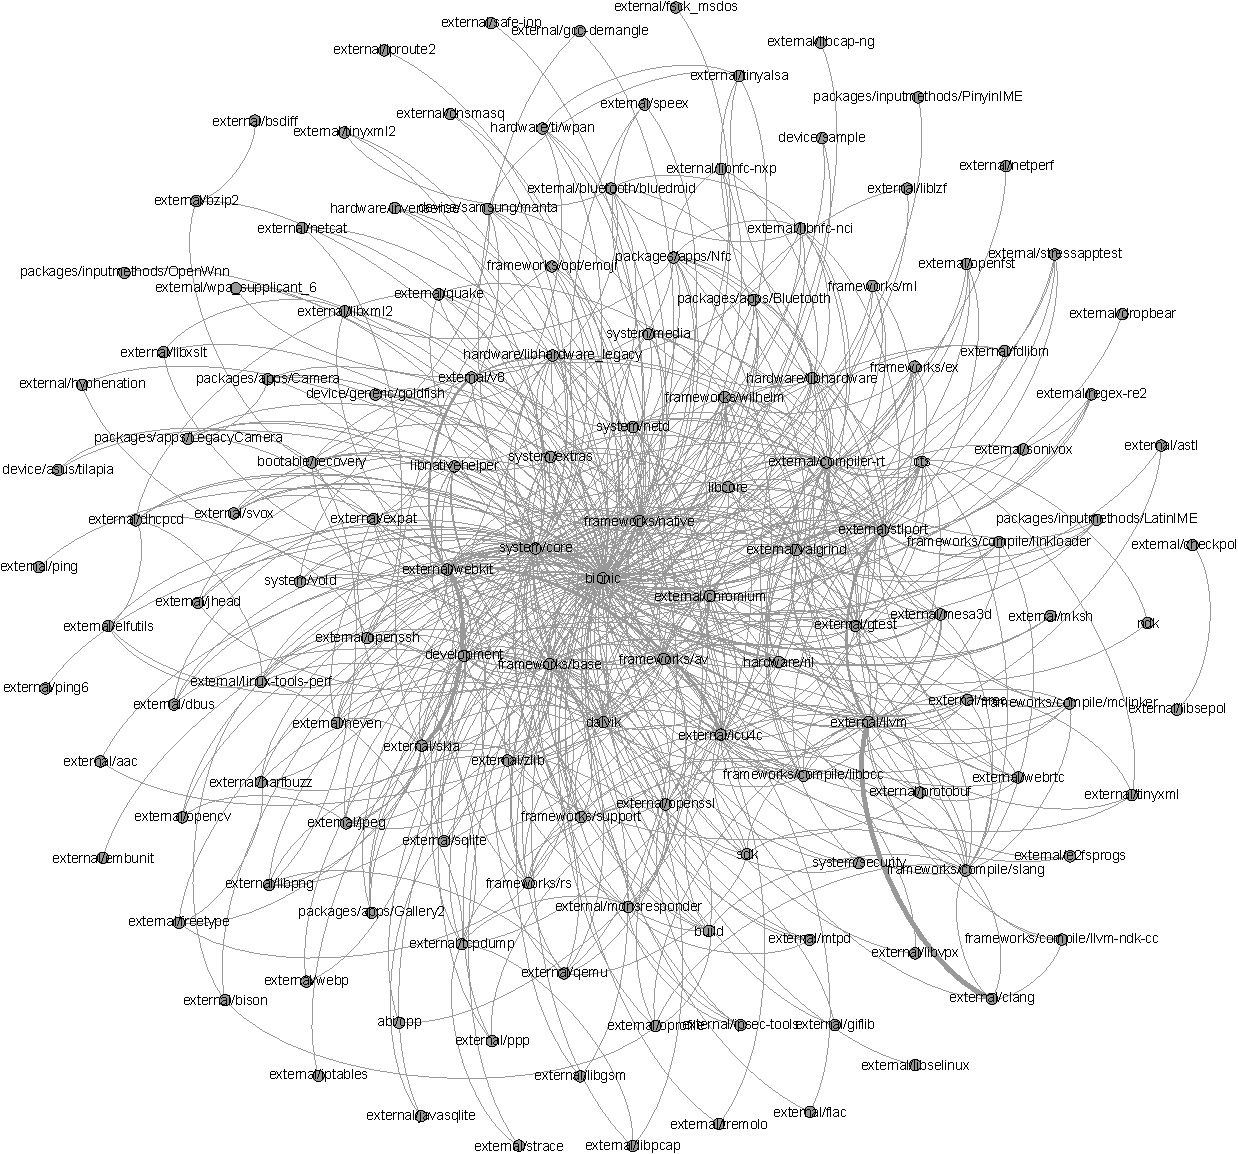
\includegraphics[width=0.9\linewidth]{callgraph.pdf}
   \caption{Граф межпакетных вызовов ОС Android 4.2}\label{pic:callgraph}
\end{figure}

\section{Методика тестирования}

Для тестирования использовался сервер, конфигурация которого описана в таблице \ref{table:test-server}:

\begin{table} [htbp]
  \centering
  \parbox{15cm}{\caption{Характеристики тестового стенда}\label{table:test-server}}
%  \begin{center}
  \begin{tabular}{| p{0.6\linewidth} || p{0.3\linewidth} |}
  \hline
  \hline
  Характеристика   & Значение \\
  \hline
  \hline
  Модель процессора   & Intel Xeon E5-2600 2.60 ГГц \\
  \hline
  Количество физических процессоров & 2   \\
  \hline
  Количество физических ядер процессора      & 8    \\
  \hline
  Количество виртуальных ядер процессора  & 16 (Hyper-Threading)   \\
  \hline
  Количество виртуальных ядер системы & 32   \\
  \hline
  Объём оперативной памяти & 96 Гб \\
  \hline
  Тип оперативной памяти & DDR3 \\
  \hline
  \hline
  \end{tabular}
%  \end{center}
\end{table}

Процессы анализаторов запускались параллельно на всех виртуальных процессорах. Время анализа измерялось от момента старта фазы анализа до момента завершения последнего процесса анализатора и выдачи финального отчёта.

В качестве базовой версии Clang Static Analyzer использовалась версия 3.4.1.

Анализатор (Clang Static Analyzer) имеет ряд настроек, непосредственно влияющих как на качество анализа, так и на его время. Ниже в таблице \ref{table:test-settings} перечислены опции анализатора, при которых производилось сравнение.

\begin{table} [htbp]
  \centering
  \parbox{15cm}{\caption{Тестовые настройки анализатора}\label{table:test-settings}}
%  \begin{center}
  \begin{tabular}{| p{0.35\linewidth} || p{0.35\linewidth} | p{0.2\linewidth} |}
  \hline
  \hline
  Имя параметра  & Назначение параметра & Значение \\
  \hline
  \hline
  \texttt{mode}   & Режим анализа. Влияет на максимальный размер функции, для которой выполняется анализ вложенного вызова & \texttt{deep} \\
  \hline
  \texttt{c++-inlining} & Анализ вызовов членов классов (C++) & \texttt{destructors}   \\
  \hline
  \texttt{cfg-temporary-dtors}   & Анализ вызовов деструкторов временныз объектов  & \texttt{false}    \\
  \hline
  \texttt{c++-stdlib-inlining} & Анализ вызовов стандартной библиотеки C++ & \texttt{true}   \\
  \hline
  \texttt{ipa-always-inline-size} & Размер функций, для которых всегда выполняется МПА & 3   \\
  \hline
  \texttt{c++-allocator-inlining} & Анализ аллокаторов (C++) & \texttt{false}   \\
  \hline
  \texttt{c++-template-inlining} & Анализ шаблонов функций (C++) & \texttt{true}   \\
  \hline
  \texttt{c++-container-inlining} & Анализ контейнерных классов (C++) & \texttt{true}   \\
  \hline
  \texttt{c++-shared\_ptr-inlining} & Анализ указателей \texttt{shared\_ptr} (C++) & \texttt{false}   \\
  \hline
  \texttt{max-times-inline-large} & Максимальное количество анализа вложенного вызова функции & 32   \\
  \hline
  \texttt{max-nodes} & Максимальное количество анализируемых узлов графа выполнения функции & \textit{варьируется}   \\
  \hline
  \hline
  \end{tabular}
%  \end{center}
\end{table}

Параметр \texttt{max-nodes} непосредственно влияет на полноту анализа, поэтому в дальнейшем измерения будут проходить с его учётом. Он станет одним из варьируемых параметров.

\section{Тестирование покрытия и производительности}

В качестве критерия производительности при сравнении межпроцедурного анализа методом встраивания и методом резюме можно взять количество узлов графа выполнения, обрабатываемых в единицу времени. Каждому оператору программы обычно соответствует 4--5 узлов графа выполнения. Данный параметр может использоваться для режима встраивания непосредственно, однако для режима резюме он не отражает реальной производительности системы, поскольку каждому из узлов применения резюме в результирующем графе выполнения соответствует полноценный путь внутри одной или нескольких функций. Однако, количество узлов графа, соответствующих узлам применения резюме, можно вычислить рекурсивно, способом, схожим со способом построения отчёта при вложенном вызове функции: 

\begin{enumerate}
 \item Установить начальный счётчик узлов \texttt{cnt} = 0, $Proceed = \varnothing$~--- набор учтённых узлов 
 \item Для всех заданных конечных точек графа выполнения выполнить шаги 3 и 4.
 \item Пусть $N$~--- узел применения резюме, $M$~--- узел графа выполнения функции, на который хранится указатель в $N$.
 \item Пока $M$~--- не корневой узел графа выполнения, и $M$ не учтён:
  \begin{enumerate}
   \item Увеличить \texttt{cnt} на 1
   \item Добавить $M$ в $Proceed$
   \item Если $M$~--- узел применения резюме, выполнить для $M$ шаги алгоритма 1--3
   \item Установить $M$ равным первому родительскому узлу $M$
  \end{enumerate}
\end{enumerate}

Таким образом, можно осуществить подсчёт количества \textit{эквивалентных} узлов графа выполнения, обрабатываемых в единицу времени. Для графа верхнего уровня вместо списка конечных узлов используется список всех узлов графа, поскольку часть ветвей выполнения графа верхнего уровня анализируется не полностью.

При измерениях необходимо учитывать, что часть времени расходуется не анализатором на анализ кода программы, а компилятором~--- на разбор исходного файла и построение синтаксического дерева. Данные затраты не меняются от прогона к прогону и составляют, в среднем, 7 минут, и это время должно быть вычтено из общего времени анализа.

Результаты измерения нижней границы для ОС Android для внутримодульного и межмодульного анализа в различных режимах анализа представлены в таблицах \ref{table:time-nodes-single} и \ref{table:time-nodes-xtu} соответственно.

\begin{table}
%\setlength{\tabcolsep}{4pt}
\renewcommand{\arraystretch}{1.2}
\begin{tabular}{| p{0.2\linewidth} | p{0.13\linewidth} | p{0.35\linewidth} | p{0.18\linewidth} |} 
\hline
Лимит количества узлов & Время анализа & Количество проанализированных узлов графа & Узлов графа в~секунду \\
\hline
\multicolumn{4}{|c|}{Метод встраивания} \\
\hline
\hline
8000      &   0:11       & $2,70 \cdot 10^8$  & $1,12 \cdot 10^6$ \\
\hline
16000     &   0:17       & $5,00 \cdot 10^8$  & $8,33 \cdot 10^5$ \\
\hline
32000     &   0:28       & $9,25 \cdot 10^8$  & $7,34 \cdot 10^5$ \\
\hline
64000     &   0:50       & $1,72 \cdot 10^9$  & $6,66 \cdot 10^5$ \\
\hline
128000    &   1:30       & $3,21 \cdot 10^9$  & $6,44 \cdot 10^5$ \\
\hline
256000    &   2:51       & $6,01 \cdot 10^9$  & $6,10 \cdot 10^5$ \\
\hline
512000    &   5:27       & $1,13 \cdot 10^{10}$  & $5,89 \cdot 10^5$ \\
\hline
\hline
\multicolumn{4}{|c|}{Метод резюме} \\
\hline
\hline
2000      &   0:09:30       & $1,94 \cdot 10^9$  & $1,29 \cdot 10^7$ \\
\hline
4000      &   0:12       & $3,90 \cdot 10^9$  & $1,30 \cdot 10^7$ \\
\hline
8000      &   0:19       & $8,49 \cdot 10^9$  & $1,18 \cdot 10^7$ \\
\hline
16000     &   0:32       & $1,68 \cdot 10^{10}$  & $1,12 \cdot 10^7$ \\
\hline
32000     &   0:52       & $3,31 \cdot 10^{10}$  & $1,22 \cdot 10^7$ \\
\hline
64000     &   1:38       & $6,70 \cdot 10^{10}$  & $1,22 \cdot 10^7$ \\
\hline
128000    &   3:00       & $1,37 \cdot 10^{11}$  & $1,32 \cdot 10^7$ \\
\hline
\hline

\end{tabular}
\caption{Результаты измерений количества узлов графа, обрабатываемых в единицу времени, при внутримодульном анализе для методов встраивания и резюме} \label{table:time-nodes-single}
\end{table}



\begin{table}
\renewcommand{\arraystretch}{1.2}
\begin{tabular}{| p{0.2\linewidth} | p{0.13\linewidth} | p{0.35\linewidth} | p{0.18\linewidth} |} 
\hline
Лимит количества узлов & Время анализа & Количество проанализированных узлов графа & Узлов графа в~секунду \\
\hline
\multicolumn{4}{|c|}{Метод встраивания} \\
\hline
\hline
8000      &   0:26       & $2,38 \cdot 10^8$  & $2,09 \cdot 10^5$ \\
\hline
16000     &  0:33        & $4,44 \cdot 10^8$  & $2,85 \cdot 10^5$ \\
\hline
32000     &  0:47        & $8,27 \cdot 10^8$  & $3,45 \cdot 10^5$ \\
\hline
64000     &  1:13        & $1,54 \cdot 10^9$  & $3,89 \cdot 10^5$ \\
\hline
128000    &   2:07       & $2,89 \cdot 10^9$  & $4,01 \cdot 10^5$ \\
\hline
256000    &   3:56       & $5,43 \cdot 10^8$  & $3,95 \cdot 10^5$ \\
\hline
\hline
\multicolumn{4}{|c|}{Метод резюме} \\
\hline
\hline
2000      &   0:28       & $1,88 \cdot 10^9$  & $1,49 \cdot 10^6$ \\
\hline
4000      &   0:41       & $3,80 \cdot 10^9$  & $1,86 \cdot 10^6$ \\
\hline
8000      &   0:53       & $8,23 \cdot 10^9$  & $2,98 \cdot 10^6$ \\
\hline
16000     &  1:23        & $1,64 \cdot 10^{10}$  & $3,59 \cdot 10^6$ \\
\hline
32000     &  2:18        & $3,23 \cdot 10^{10}$  & $4,11 \cdot 10^6$ \\
\hline
64000     &  4:41        & $6,52 \cdot 10^{10}$ & $3,97 \cdot 10^6$ \\
\hline
\hline

\end{tabular}
\caption{Результаты измерений количества узлов графа, обрабатываемых в единицу времени, при межмодульном анализе для метода резюме} \label{table:time-nodes-xtu}

\end{table}


\begin{figure}[h]
   \centering
   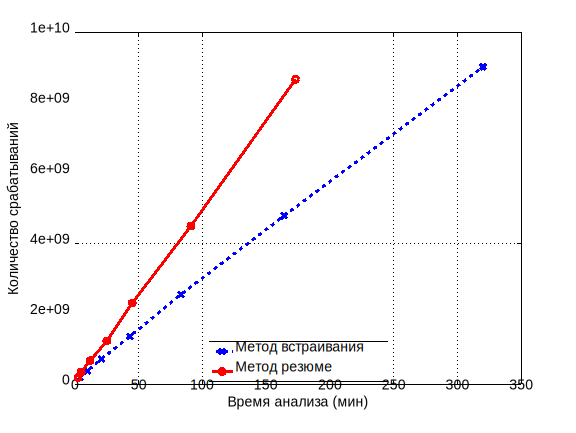
\includegraphics[width=0.8\linewidth]{single-nodes}
   \caption{Количество анализируемых узлов графа при внутримодульном анализе для методов встраивания и резюме}\label{pic:single-nodes}
\end{figure}

\begin{figure}[h]
   \centering
   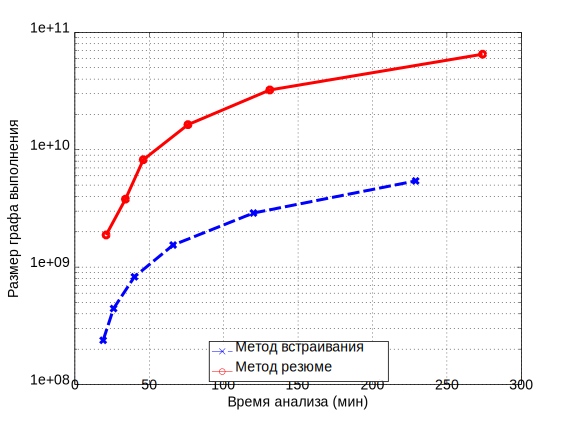
\includegraphics[width=0.8\linewidth]{xtu-nodes}
   \caption{Количество анализируемых узлов графа при межмодульном анализе для методов встраивания и резюме}\label{pic:xtu-nodes}
\end{figure}


\section{Обнаружение дефектов}

Основной целью прогона статического анализатора является обнаружение дефектов. Поэтому, помимо покрытия анализа, необходимо проанализировать сообщения о дефектах, выданные анализатором при выполнении анализа программы.

Для проверки использовались проверяющие модули ConstModifiedChecker и IntegerOverflowChecker, поскольку срабатывания прочих проверяющих модулей на данной кодовой базе были единичными или отсутствовали вообще. При сравнении результатов анализа необходимо учитывать, что анализатор может выдавать отчёты на одном и том же операторе при анализе различных путей выполнения программы. Отчёты, относящиеся к одному оператору (точнее, к одной и той же позиции в исходном коде) и к одному и тому же проверяющему модулю, обычно унифицируются, поскольку пользователю не имеет смысла изучать один и тот же дефект несколько раз. С другой стороны, общее количество срабатываний без учёта унификации может коррелировать с покрытием анализатором путей программы. Следовательно, имеет смысл рассматривать как уникальные срабатывания анализатора, так и срабатывания без унификации.


\begin{table}
%\setlength{\tabcolsep}{4pt}
\renewcommand{\arraystretch}{1.2}
\begin{tabular}{| p{0.2\linewidth} | p{0.13\linewidth} | p{0.16\linewidth} | p{0.18\linewidth} |  p{0.16\linewidth} |} 
\hline
Лимит количества узлов & Время анализа & Отчётов анализатора & Уникальных отчётов & Отчётов в~секунду \\
\hline
\multicolumn{5}{|c|}{Метод встраивания} \\
\hline
\hline
8000      &   0:11       & 81861  & 1506 & 6,28 \\
\hline
16000     &   0:17       & 164551  & 1616 & 2,70 \\
\hline
32000     &   0:28       & 318558  & 1703 & 1,35 \\
\hline
64000     &   0:50       & 624176  & 1771 & 0,69 \\
\hline
128000    &   1:30       & 1199886  & 1828 & 0,37 \\
\hline
256000    &   2:51       & 2242228  & 1895 & 0,19 \\
\hline
512000    &   5:27       & 4189537  & 1933 & 0,10 \\
\hline
\hline
\multicolumn{5}{|c|}{Метод резюме} \\
\hline
\hline
2000      &   0:09:30    & 209038  & 1457 & 9,71 \\
\hline
4000      &   0:12       & 366782  & 1591 & 5,30 \\
\hline
8000      &   0:19       & 658994  & 1696 & 2,36 \\
\hline
16000     &   0:32       & 1174869  & 1773 & 1,18 \\
\hline
32000     &   0:52       & 2358712  & 1834 & 0,68 \\
\hline
64000     &   1:38       & 4465568  & 1886 & 0,35 \\
\hline
128000    &   3:00       & 8661287  & 1911 & 0,19 \\
\hline
\hline

\end{tabular}
\caption{Количество отчётов о дефектах при внутримодульном анализе для методов встраивания и резюме} \label{table:time-defect-single}
\end{table}

\begin{table}
%\setlength{\tabcolsep}{4pt}
\renewcommand{\arraystretch}{1.2}
\begin{tabular}{| p{0.2\linewidth} | p{0.13\linewidth} | p{0.16\linewidth} | p{0.18\linewidth} |  p{0.16\linewidth} |} 
\hline
Лимит количества узлов & Время анализа & Отчётов анализатора & Уникальных отчётов & Отчётов в~секунду \\
\hline
\multicolumn{5}{|c|}{Метод встраивания} \\
\hline
\hline
8000      &   0:26       & 79019  & 1769 & 1,55 \\
\hline
16000     &  0:33        & 159236  & 1907 & 1,22 \\
\hline
32000     &  0:47        & 308988  & 2048 & 0,85 \\
\hline
64000     &  1:13        & 606951  & 2143 & 0,54 \\
\hline
128000    &   2:07       & 1168253  & 2194 & 0,30 \\
\hline
256000    &   3:56       & 2185124  & 2281 & 0,17 \\
\hline
\hline
\multicolumn{5}{|c|}{Метод резюме} \\
\hline
\hline
2000      &   0:28       & 207120  & 1715 & 1,36 \\
\hline
4000      &   0:41       & 358641  & 1900 & 0,93 \\
\hline
8000      &   0:53       & 653184  & 2066 & 0,75 \\
\hline
16000     &  1:23        & 1159685  & 2275 & 0,50 \\
\hline
32000     &  2:18        & 2348704  & 2326 & 0,30 \\
\hline
64000     &  4:41        & 4487512  & 2430 & 0,15 \\
\hline
\hline

\end{tabular}
\caption{Количество отчётов о дефектах при межмодульном анализе для методов встраивания и резюме} \label{table:time-defect-xtu}
\end{table}

\begin{figure}[h]
   \centering
   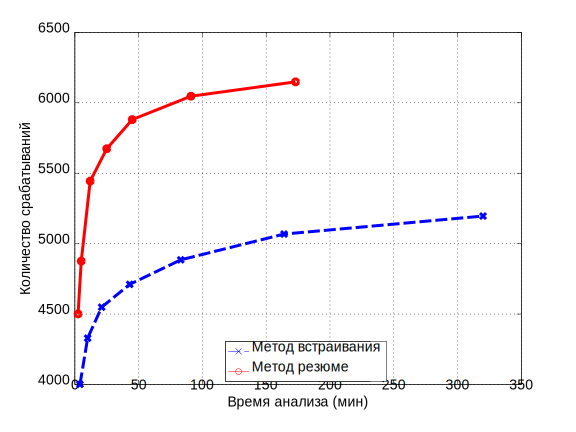
\includegraphics[width=0.8\linewidth]{single-non-unique}
   \caption{Количество найденных дефектов при внутримодульном анализе для методов встраивания и резюме}\label{pic:single-non-unique}
\end{figure}


\begin{figure}[h]
   \centering
   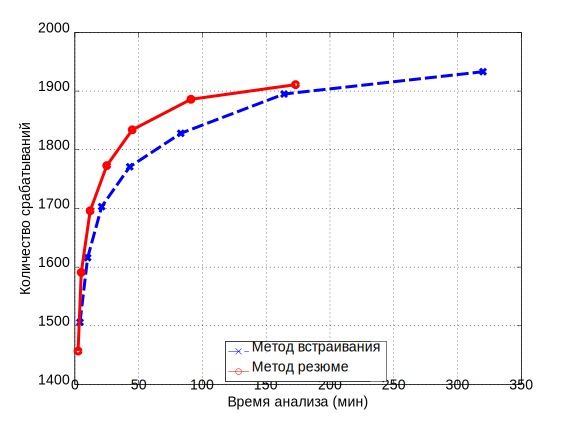
\includegraphics[width=0.8\linewidth]{single-unique}
   \caption{Количество уникальных дефектов при внутримодульном анализе для методов встраивания и резюме}\label{pic:single-unique}
\end{figure}



\begin{figure}[h]
   \centering
   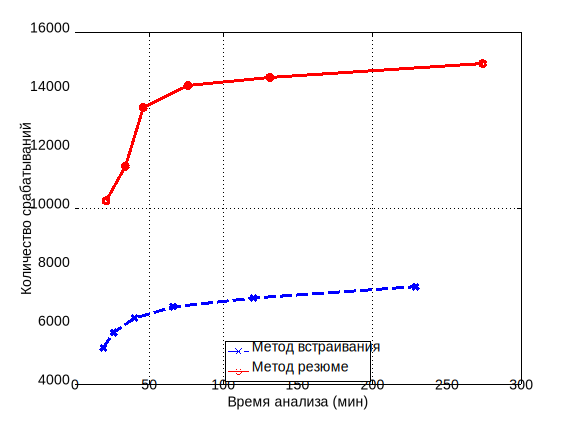
\includegraphics[width=0.8\linewidth]{xtu-non-unique}
   \caption{Количество найденных дефектов при межмодульном анализе для методов встраивания и резюме}\label{pic:xtu-non-unique}
\end{figure}


\begin{figure}[h]
   \centering
   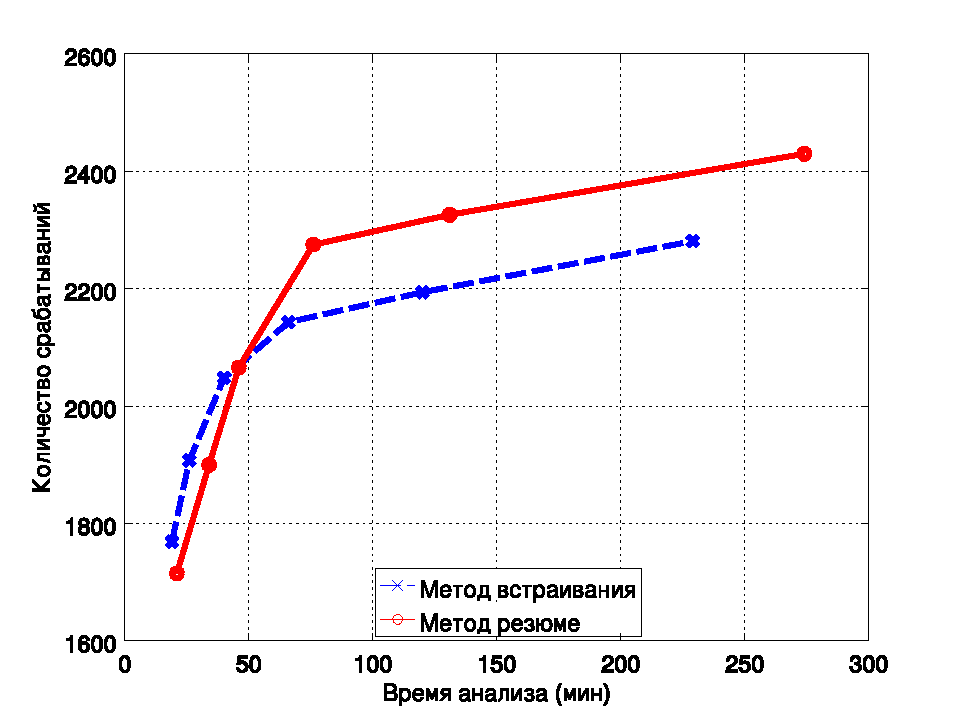
\includegraphics[width=0.8\linewidth]{xtu-unique}
   \caption{Количество уникальных дефектов при межмодульном анализе для методов встраивания и резюме}\label{pic:xtu-unique}
\end{figure}

Часть срабатываний была проверена вручную. По результатам проверки построена таблица \ref{table:defect-quality-single}. Как видно из таблицы, качество анализа у использованных проверяющих модулей при использовании метода резюме осталось примерно таким же, как и при использовании метода встраивания. Это свидетельствует об эквивалентности двух методов проверки для этих проверяющих модулей. Кроме того, часть срабатываний, обнаруженных при межмодульном анализе, также является межмодульными, т.~е. их трасса включает в себя несколько файлов исходного кода. Эти срабатывания не могли быть обнаружены при внутримодульном анализе, и это свидетельствует об увеличении полноты анализа.

\begin{table}
%\setlength{\tabcolsep}{4pt}
\renewcommand{\arraystretch}{1.2}
\begin{tabular}{| p{0.1\linewidth} | p{0.13\linewidth} | p{0.2\linewidth} | p{0.09\linewidth} |  p{0.09\linewidth} |  p{0.1\linewidth} |  p{0.11\linewidth} |} 
\hline
Метод ИПА & \texttt{max-nodes} & Уникальных срабатываний & TP & FP & Unclear & Качество \\
\hline
\multirow{7}{*}{\rotatebox[origin=c]{90}{\parbox{\linewidth}{Метод\\встраивания}}}
& 8000      &   1506       & 203  & 13 & 29 & 82\% \\
\cline{2-7}
&16000     &  1616        & 206  & 14 & 30 & 82\% \\
\cline{2-7}
&32000     &  1703        & 212  & 14 & 31 & 82\% \\
\cline{2-7}
&64000     &  1771        & 220  & 15 & 34 & 81\% \\
\cline{2-7}
&128000    &   1828       & 222  & 16 & 34 & 81\% \\
\cline{2-7}
&256000    &   1895       & 223  & 18 & 34 & 81\% \\
\cline{2-7}
&512000    &   1933       & 229  & 18 & 34 & 81\% \\
\hline
\hline
\multirow{7}{*}{\rotatebox{90}{Метод резюме}}
& 2000      &   1457       & 150  & 12 & 21 & 83\% \\
\cline{2-7}
&4000       &   1591       & 165  & 14 & 21 & 82\% \\
\cline{2-7}
&8000       &   1696       & 168  & 14 & 21 & 83\% \\
\cline{2-7}
&16000      &  1773        & 173  & 14 & 21 & 83\% \\
\cline{2-7}
&32000      &  1834        & 181  & 14 & 21 & 82\% \\
\cline{2-7}
&64000      &  1886        & 182  & 14 & 25 & 82\% \\
\cline{2-7}
&128000     &   1911       & 182  & 15 & 25 & 81\% \\
\hline
\hline

\end{tabular}
\caption{Количество отчётов о дефектах при внутримодульном анализе для методов встраивания и резюме} \label{table:defect-quality-single}
\end{table}



\begin{table}
%\setlength{\tabcolsep}{4pt}
\renewcommand{\arraystretch}{1.2}
\begin{tabular}{| p{0.1\linewidth} | p{0.13\linewidth} | p{0.2\linewidth} | p{0.09\linewidth} |  p{0.09\linewidth} |  p{0.1\linewidth} |  p{0.11\linewidth} |} 
\hline
Метод ИПА & \texttt{max-nodes} & Уникальных срабатываний & TP & FP & Unclear & Качество \\
\hline
\multirow{7}{*}{\rotatebox[origin=c]{90}{\parbox{\linewidth}{Метод\\встраивания}}}
& 8000      &   1769       & 180  & 12 & 29 & 81\% \\
\cline{2-7}
&16000     &  1907        & 184  & 12 & 30 & 81\% \\
\cline{2-7}
&32000     &  2048        & 186  & 14 & 30 & 80\% \\
\cline{2-7}
&64000     &  2143        & 193  & 13 & 32 & 81\% \\
\cline{2-7}
&128000    &   2194       & 194  & 15 & 32 & 80\% \\
\cline{2-7}
&256000    &   2281       & 195  & 15 & 33 & 80\% \\
\hline
\hline
\multirow{7}{*}{\rotatebox[origin=c]{90}{Метод резюме}}
& 2000      &   1715       & 146  & 9 & 18 & 84\% \\
\cline{2-7}
&4000       &   1900       & 159  & 10 & 17 & 85\% \\
\cline{2-7}
&8000       &   2066       & 163  & 12 & 18 & 84\% \\
\cline{2-7}
&16000      &  2275        & 165  & 14 & 18 & 83\% \\
\cline{2-7}
&32000      &  2326        & 169  & 13 & 18 & 84\% \\
\cline{2-7}
&64000      &  2430        & 177  & 13 & 21 & 83\% \\
\hline
\hline

\end{tabular}
\caption{Количество отчётов о дефектах при межмодульном анализе для методов встраивания и резюме} \label{table:defect-quality-xtu}
\end{table}

\section{Общие выводы по результатам тестирования}

Данные, собранные в результате проведённого тестирования, позволяют сделать как ряд выводов в отношении настоящей работы, так и некоторые выводы  общего характера относительно проблемы статического анализа. Эти выводы касаются основных целей работы~--- увеличения производительности анализа методом символьного выполнения при сохранении его качества, а также возможности поиска дефектов, не локализованных в одной единице трансляции. 

Анализируя результаты тестирования по покрытию, можно констатировать увеличение количества анализируемых узлов графа в единицу времени на порядок (около 15--20 раз). Соответствующим образом растёт и количество обрабатываемых операторов программы, а также покрытие анализа. Это может считаться очень хорошим результатом. Количество путей с обнаруживаемыми дефектами также растёт (которое представляет собой общее количество найденных дефектов), что дополнительно свидетельствует в пользу возросшего покрытия анализа. Вместе с тем, зависимость покрытия от времени осталась асимптотически линейной. Это свидетельствует о том, что уйти от экспоненциальной сложности анализа всё же не удалось, несмотря на наблюдаемое увеличение производительности.

Вместе с увеличением покрытия закономерно увеличивается и количество уникальных дефектов, находимых в единицу времени. График поиска уникальных дефектов при внутримодульном анализе имеет вид кривой, сходящейся к отметке приблизительно в 2000 дефектов. Эта сходимость объясняется тем, что внутри одной единице трансляции количество потенциально обнаруживаемых дефектов ограничено, и при прогонах анализатора мы приближаемся к верхнему пределу количества обнаруживаемых дефектов. При межмодульном анализе график имеет схожую форму, однако сходимость меньше, что объясняется резко увеличившимся количеством путей выполнения в сочетании с линейной асимптотикой производительности. Однако, и при межмодульном анализе скорость поиска дефектов при использовании метода резюме заметно выше.

Как можно наблюдать по результатам тестирования, при межмодульном анализе затрачиваемое время увеличивается примерно в три раза при использовании обоих методов МПА. Причиной этого является, во-первых, увеличение времени, затрачиваемого на дисковый ввод-вывод при загрузке дополнительных синтаксических деревьев и обращении к поиску определений загружаемых функций; часть времени также затрачивается на объединение синтаксических деревьев. Во-вторых, в текущей версии межмодульного анализа на данный момент не реализовано повторное использование результатов анализа вызываемых функций при анализе различных единиц трансляции. Для решении этой проблемы можно предложить два способа:
\begin{enumerate}
 \item Объединение синтаксических деревьев единиц трансляции, которые используют общие вызываемые функции. Данный подход, хотя и не слишком сложен в реализации, на практике имеет два крупных недостатка. Во-первых, его использование приводит к усложнению управления памятью анализатора, вызываемое необходимостью длительно хранить в памяти и удалять резюме функций, а также прогнозировать, какие резюме будут использованы, а какие~--- нет. Во-вторых, данный подход усложняет распараллеливание и, соответственно, масштабирование анализатора.
 \item Лучшим вариантом является сериализация резюме и его сохранение на диск и последующее чтение. В качестве недостатка подхода стоит отметить увеличение количества операций дискового ввода-вывода. Кроме того, размер резюме слабо прогнозируем, и затраты на дисковые операции трудно определить заранее.
\end{enumerate}

Эта проблема станет одним из направлений последующих исследований, поскольку её решение должно значительно повысить производительность межмодульного анализа.

Распределение находимых дефектов по времени анализа заслуживает дополнительного рассмотрения и соответствующих выводов. Как следует из полученных данных, значительное количество дефектов может быть найдено в течение первого часа анализа. Более того, около половины находимых дефектов может быть найдено в первые десять минут анализа при минимальной глубине анализа. Из данного наблюдения можно сделать ряд интересных выводов.

\begin{enumerate}
 \item Поиск значительного количества дефектов не требует применения специальных аппаратных средств и может быть произведён с использованием непосредственно персонального компьютера, доступного разработчику программы.
 \item Высокая скорость поиска первых дефектов может означать высокую эффективность анализа программного кода <<на лету>>. В частности, эффективной для поиска дефектов может стать интеграция анализатора со средой разработки. Это потенциально может позволить быстрое обнаружение и исправление значительной части дефектов даже при небольшой глубине анализа и минимальном фоновом использовании ресурсов компьютера.
 \item Малая глубина анализа большого количества дефектов свидетельствует об их высокой пространственной локализации в рамках одной или двух функций. Данное наблюдение позволяет подтвердить существующее предположение о том, что многие дефекты могут быть достаточно эффективно обнаружены при инспекции кода, поскольку данный объём кода может быть достаточно подробно рассмотрен одним разработчиком в процессе инспекции.
\end{enumerate}

Вместе с тем, данные выводы нисколько не умаляют значимости проведения глубокого анализа программ, и, более того, подтверждают её. Глубокий анализ требует значительного времени для проведения, однако позволяет находить дефекты, которые трудно обнаруживаются другими способами, в том числе проверкой кода непосредственно человеком. Дефекты, трасса обнаружения которых включает несколько функций, обычно обнаруживаются уже в результате отладки, а не на стадии разработки, что повышает ценность их раннего обнаружения. Если же трасса дефектов затрагивает несколько отдельных компонентов, то данная проблема может быть обнаружена без использования специальных средств не ранее, чем на стадии интеграционного тестирования, что увеличивает затраты на поиск и исправление дефекта. Таким образом, статический анализ, в том числе, межмодульный анализ, является крайне перспективным дополнением к процессу разработки программного обеспечения.
